\section{Logic Circuits}

\subsection*{A Half Adder}

A \emph{half adder} demonstrates the way in which computer logic gates can correctly add (binary) numbers, though here it can add only two \emph{binary digits} (``bits''). Thus, each half adder can only count to \emph{two}, but that is enough!  Long cascades of half adders and \emph{full adders} enable computers to count large numbers. Below, see two examples of half adders. The second example replaces the XOR gate with a series of simpler gates, but the results are the same. Each half adder takes two bits and adds them, passing on the bits for further work or as an answer itself.

\bigskip

\begin{figure}[!ht]
\begin{center}
\begin{tabular}{m{3.25in} m{2.0in}}

\begin{circuitikz}

\draw
	(4,2) node[xor port](xorGate) {} %xor gate
	(4.2,3.0) node[left] {$XOR$} % XOR label
	(0,2.25) to[short](xorGate.in 1) %xor A wiring
	(0,1.75) to[short](xorGate.in 2) %xor B wiring
	(0,2.25) node[ocirc] {} %A node
	(0,2.3) node[left] {{\color{red}$A$}} %A label
	(0,1.75) node[ocirc] {} %B node
	(0,1.75) node[left] {{\color{red}$B$}} %B label
	(xorGate.out) to[short](5,2) %S output wiring
	(5,2) node[ocirc] {} %S node
	(5,2) node[right] {{\color{red}$Sum$}} %S label
	(4,0) node[and port](andGate) {} %AND gate
	(4.2,-1.0) node[left] {$AND$} % AND label
	(1,2.25) node[circ] {}
	(1.5,1.75) node[circ] {}
	(1.5,1.75) |- (andGate.in 1)
	(1,2.25) |- (andGate.in 2)
	(andGate.out) to[short](5,0) %C output wiring
	(5,0) node[ocirc] {} %C node
	(5,0) node[right] {{\color{red}$Carry$}} %C label
;
\end{circuitikz}


&

\begin{tabular}{ll | cc | c}
\multicolumn{5}{c}{\textbf{Truth Table}}\\
\hline\\[\negsep]
\textbf{A} & \textbf{B} & \textbf{Sum} & \textbf{Carry} & \textbf{Decimal}\\
\hline
0 & 0 & 0 & 0 & 0 \\
1 & 0 & 1  & 0 & 1 \\
0 & 1 & 1  & 0 & 1 \\
1 & 1 & 0  & 1 & 2 \\
\hline
\end{tabular}

\\

\end{tabular}

\caption{A half-adder circuit. It adds two bits together. If the result is larger than 1, the ``carry" signal is high.}
\end{center}
\end{figure}


\begin{figure}[!hb]
\begin{center}

\begin{circuitikz}

\draw
% Inputs:
	(2,4.25) node[american not port](nota){}   % not gate #1 input
	(2,1.75) node[american not port](notb){}   % not gate #2 input

	(0,5.5) node[ocirc](anode) {} %A node
	(0.25,6.0) node[left] {{\color{red}$A$}} %A label
	
	(0.75,5.5) node[ocirc](bnode) {} %B node
	(1.1,6.0) node[left] {{\color{red}$B$}} %B label
	
% AND gates:
	(4.5,3.75) node[american and port](andGate1) {} % AND gate #1 
	(4.5,2.25) node[american and port](andGate2) {} % AND gate #2 
	(5,0) node[american and port](andGate3) {} % AND gate #3

% OR gate:
	(7.0,3) node[american or port](orGate) {}

% From the NOT gates out to the AND gates and OR gate:
	(nota.out) to[short](andGate1.in 1) % S output wiring goes into andGate1.in 1
	(notb.out) to[short](andGate2.in 2) % S output wiring goes into andGate1.in 2

	(0,3.5) node[circ](atoand1){}
	(atoand1) to [short](andGate1.in 2)

	(andGate1.out) to [short](5.0,3.75)
	(5.0,3.75)  |- (orGate.in 1)

	(andGate2.out) to [short](5.0,2.25)
	(5.0,2.25)  |- (orGate.in 2)

	(0.75,4.25) node[circ](btonot1){}	
	(bnode) |- (nota.in)

	(0,5.5) |- (notb.in)
	(0,1.75) node[circ](atonot2){}
	(atonot2) |- (andGate3.in 2)

% B input line nets:
	(0.75,4.25) to [short](0.75,2.5)
	(0.75,2.52) node[circ]{}
	(0.75,2.52) |- (andGate2.in 1)
	(0.75,2.5) |- (andGate3.in 1)
	
% Output nodes:
	(8,3) node[ocirc](snode) {} %S node
	(8.25,3) node[right] {{\color{red}$Sum$}} % S label

	(5.75,0) node[ocirc](cnode) {} % C node
	(6.0,0) node[right] {{\color{red}$Carry$}} % C label

	(andGate3.out) to[short](cnode) % C output
	(orGate.out) to [short](snode) % S output 
	
% Labeling:
	(1.75,4.85) node[right] {{\footnotesize{NOT 1}}} 
	(1.75,1.15) node[right] {{\footnotesize{NOT 2}}} 
	(3.5,4.6) node[right] {{\footnotesize{AND 1}}} 
	(3.5,1.35) node[right] {{\footnotesize{AND 2}}}
	(4.5,-0.6) node[right] {{\footnotesize{AND 3}}}
	(6.5,3.7) node[right] {{\footnotesize{OR}}}
    
    ;

\end{circuitikz}

\caption{Another half-adder circuit. The XOR gate has been replaced by an equivalent circuit made up of simpler gates.}
\end{center}
\end{figure}


\subsection*{Full Adder}

This type of adder is a little more difficult to implement than a half-adder. The main difference between a half-adder and a full-adder is that the full-adder has \emph{three} inputs and two outputs. The first two inputs are A and B, just like with every half-adder, and the third input is an input carry, designated as $C_{in}$. Enabling the circuit to handle a carry \emph{in} from another adder makes it possible to add many binary orders of magnitude, since many carry-outs and carry-ins will be needed to add numbers larger than 1. Once we implement a full adder, we can string eight of them together to create a byte-wide adder and cascade the carry bit from one adder to the next.
\bigskip

\begin{figure}[!hb]
\begin{center}
\begin{circuitikz}
\draw
% Inputs and outputs:
	(0,4.25) node[ocirc](ain) {} % A node
	(0,4.30) node[left] {{\color{red}$A$}} % A label
	
	(0,3.72) node[ocirc](bin) {} % B node
	(0,3.72) node[left] {{\color{red}$B$}} % B label

	(0,1.72) node[ocirc](cin) {} % C-in node
	(0,1.72) node[left] {{\color{red}$C_{in}$}} % C-in label

	(8.2,1.0) node[ocirc](cout) {} % C-out node
	(8.2,1.0) node[right] {{\color{red}$C_{out}$}} % C-out label

	(8.2,3.72) node[ocirc](sout) {} % S node
	(8.2,3.72) node[right] {{\color{red}$Sum$}} % S label

% Gates:
	(2.8,4.0) node[xor port](xorGate1) {} % xor gate 1
	(3.0,4.9) node[left] {$XOR_1$} % XOR_1 label

	(5.5,3.72) node[xor port](xorGate2) {} % xor gate 2
	(5.7,4.60) node[left] {$XOR_2$} % XOR_2 label 

	(2.8, 0.0) node[and port](andGate1) {} % AND gate 1
	(3.0,-1.0) node[left] {$AND_1$} % AND_1 label
 
	(5.5,2) node[and port](andGate2) {} % AND gate 2
	(5.7,1) node[left] {$AND_2$} % AND_2 label

	(7.75,1.00) node[or port](orGate1) {} % or gate
	(7.55,0.1) node[left] {$OR$} % OR label

% Tie A and B to XOR_1:
	(ain) to[short](xorGate1.in 1) 
	(bin) to[short](xorGate1.in 2)  

% Tie XOR_1 output to XOR_2 input and to AND_2 input:
	(xorGate1.out) |- (xorGate2.in 1) 
	(3.5,4.0) node[circ]{}
	(3.5,4.0) |- (andGate2.in 1)

% Tie A and B to AND_1:	
	(1.0,3.72) node[circ] {}
	(0.5,4.25) node[circ] {}
	(1.0,3.72) |- (andGate1.in 1)
	(0.5,4.25) |- (andGate1.in 2)

% Tie C-in to AND_2 and XOR_2:
	(cin) |- (andGate2.in 2)
	(3.0,1.72) node[circ]{}
	(3.0,1.72) |- (3.0, 3.4)
	(3.0,3.40) |- (xorGate2.in 2)

% Tie AND gate outputs to the OR gate:
	(andGate2.out) |- (6,2)
	(andGate1.out) to[short](6,0)
	(6,2)   |- (orGate1.in 1)
	(6,0)   |- (orGate1.in 2)

% Outputs:
	(xorGate2.out) |- (sout) % XOR_2 to Sum
	(orGate1.out) |- (cout) % OR to Carry-out

;
\end{circuitikz}
\caption{A full-adder circuit, made up of two half-adder circuits. A full-adder enables carry-in as well as carry-out. These units can be linked together to make binary addition work even for very large numbers.}
\end{center}
\end{figure}


\begin{figure}[!ht]
\begin{center}
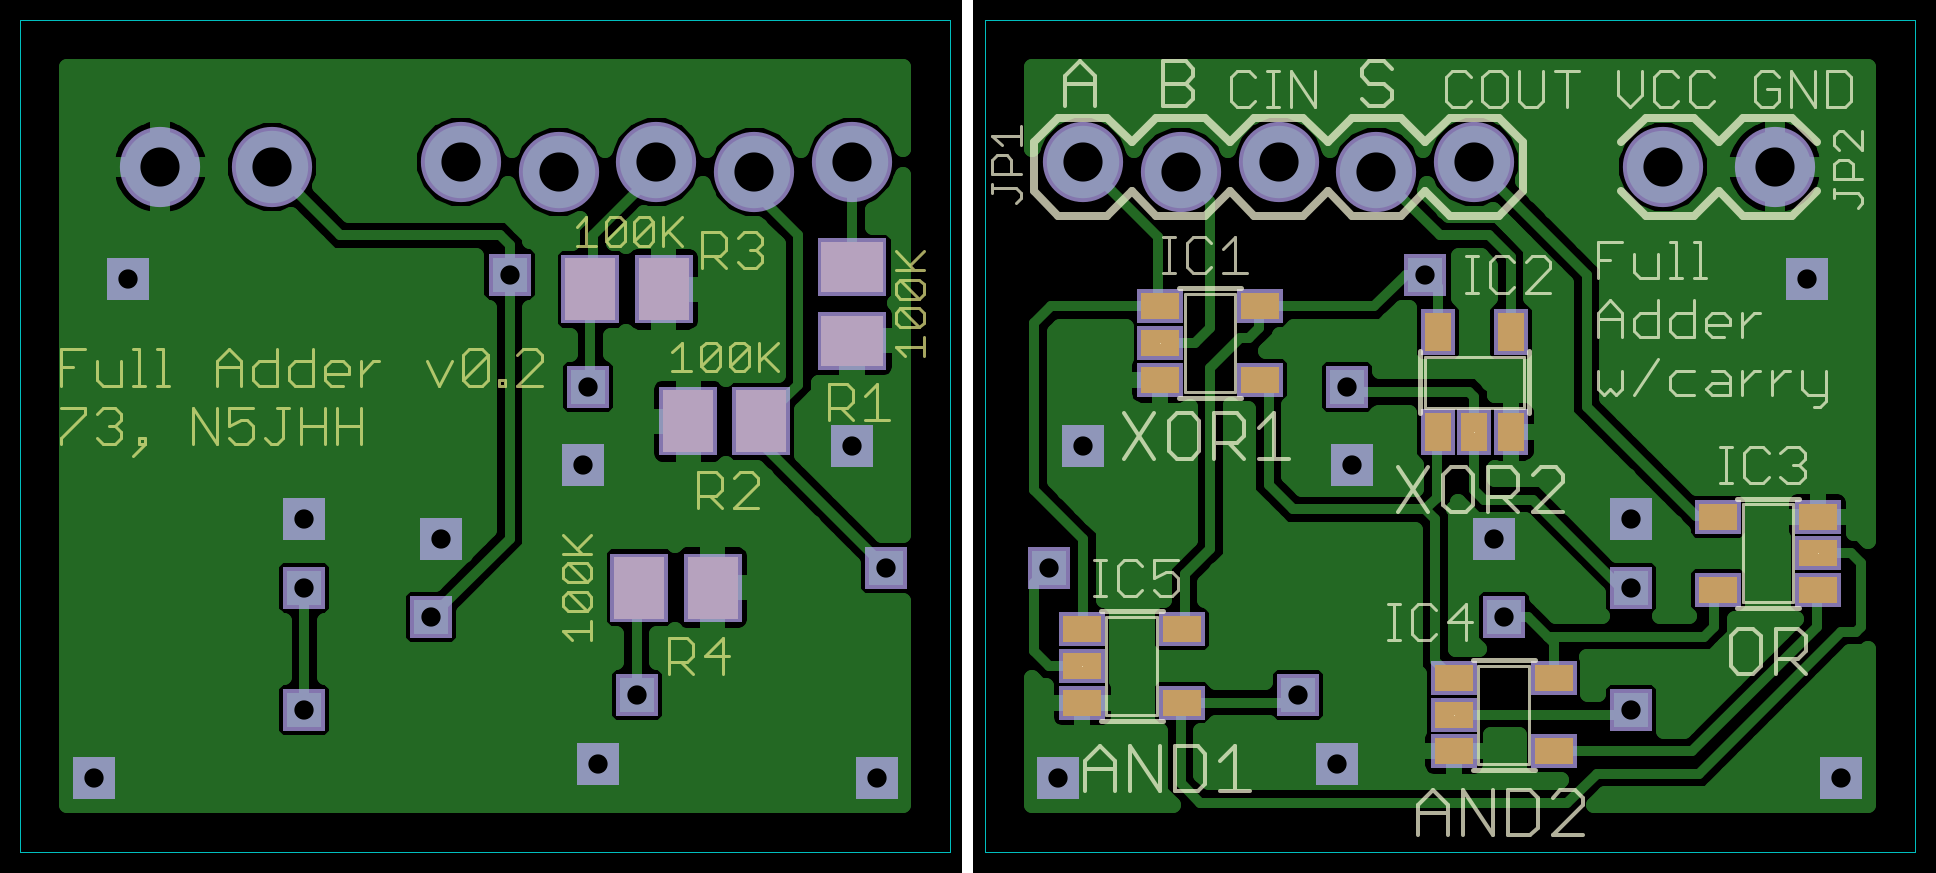
\includegraphics[scale=0.19]{FullAdderboard.png}
\caption{A full-adder circuit for adding two bits plus a carry-in digit, implemented on a small circuit board using individual integrated circuit gates instead of discrete transistors. You can see the circuits easily but the board is much simpler to work with, compared to the single-gate boards.}
\end{center}
\end{figure}




\clearpage

\subsection*{Equality}

Comparing two one-bit numbers to see if they are identical is done with XNOR gates. These gates are the same as an XOR gate passing output into a NOT gate. 

\medskip
\begin{center}

\begin{tabular}{p{2.5in} p{3.5in} }
\hline\\[\negsep]

The symbol for an XNOR gate is:

\vspace{0.25in}

\begin{circuitikz}
\draw
	(0,0) node[xnor port](xnorGate) {}
	(xnorGate.in 1) node[left] {{\color{red}$INPUT~A$}}
	(xnorGate.in 2) node[left] {{\color{red}$INPUT~B$}}
	(xnorGate.out) node[right] {{\color{red}$OUT$}}
;
\end{circuitikz}

&

\centering

The ``Truth Table" (how they behave) is: 
\vspace{0.15in}

\begin{tabular}{ll | c}
\multicolumn{3}{c}{\textbf{XNOR Gate }}\\
\multicolumn{3}{c}{\textbf{Truth Table}}\\
\hline\\[\negsep]
\textbf{A} & \textbf{B} & \textbf{OUT}\\
\hline
0 & 0 & 1  \\
1 & 0 & 0  \\
0 & 1 & 0  \\
1 & 1 & 1  \\
\hline
\end{tabular}
\\
\tabularnewline

\hline\\[\negsep]

\end{tabular}
\end{center}

\bigskip

To compare large numbers, the circuit requires an XNOR gate for each binary digit (bit) in the numbers being compared. If any XNOR gate returns zero, the numbers are not equivalent. To build all of the XNOR gates into a single yes or no answer, each XNOR output could go into a series of AND gates -- that is, since AND returns a ``yes'' only if both inputs are one, a single ``no'' prevents the AND gate from returning ``yes''. 


\begin{figure}[h!]
\begin{center}
\begin{circuitikz}

\draw

% Gates:
	(2,0.5) node[xnor port](xnorGate0) {} % xnor gate
	(1.05,1.05) node[above] {$XNOR_0$} % XNOR label

	(2,2.5) node[xnor port](xnorGate1) {} % xnor gate
	(1.05,3.1) node[above] {$XNOR_1$} % XNOR label
	
	(4.5,1.5) node[and port](andGate0) {} % AND gate 0
%	(4.1,2) node[left] {$AND_0$} % AND label

	(2,6.5) node[xnor port](xnorGate3) {} % xnor gate
	(1.05,7.05) node[above] {$XNOR_3$} % XNOR label

	(2,4.5) node[xnor port](xnorGate2) {} % xnor gate
	(1.05,5.1) node[above] {$XNOR_2$} % XNOR label
	
	(4.5,5.5) node[and port](andGate1) {} % AND gate 1
	
	(6.5,3.5) node[and port](andGate2) {} % AND gate 2


% Input nodes:
	(0,0.77) node[ocirc](ainput0) {} % A node
	(0,0.83) node[left] {{\color{red}$A_0$}} % A label

	(0,0.25) node[ocirc](binput0) {} % B node
	(0,0.22) node[left] {{\color{red}$B_0$}} % B label

	(0,2.77) node[ocirc](ainput1) {} % A node
	(0,2.75) node[left] {{\color{red}$A_1$}} % A label

	(0,2.22) node[ocirc](binput1) {} % B node
	(0,2.20) node[left] {{\color{red}$B_1$}} % B label


	(0,4.77) node[ocirc](ainput2) {} % A node
	(0,4.72) node[left] {{\color{red}$A_2$}} % A label

	(0,4.22) node[ocirc](binput2) {} % B node
	(0,4.23) node[left] {{\color{red}$B_2$}} % B label

	(0,6.77) node[ocirc](ainput3) {} % A node
	(0,6.75) node[left] {{\color{red}$A_3$}} % B label

	(0,6.22) node[ocirc](binput3) {} % B node
	(0,6.20) node[left] {{\color{red}$B_3$}} % B label

% Output nodes:

	(7.5, 3.5) node[ocirc](output){}
	(7.7, 3.75) node[above] {{\color{red}$Result$}}
	(andGate2.out) |- (output)

% Nets:
	(ainput0) |- (xnorGate0.in 1) % xor A wiring
	(binput0) |- (xnorGate0.in 2) % xor B wiring

	(ainput1) |- (xnorGate1.in 1) % xor A wiring
	(binput1) |- (xnorGate1.in 2) % xor B wiring	

	(ainput2) |- (xnorGate2.in 1) % xor A wiring
	(binput2) |- (xnorGate2.in 2) % xor B wiring

	(ainput3) |- (xnorGate3.in 1) % xor A wiring
	(binput3) |- (xnorGate3.in 2) % xor B wiring	

	(xnorGate0.out) |- (andGate0.in 2)
	(xnorGate1.out)	|- (andGate0.in 1)

	(xnorGate2.out) |- (andGate1.in 2)
	(xnorGate3.out)	|- (andGate1.in 1)

	(andGate0.out) |- (andGate2.in 2)
	(andGate1.out) |- (andGate2.in 1)

;

\end{circuitikz}

\caption{A circuit to provide a yes/no answer to the question, ``are  two four-bit numbers, A and B, equal?" Each XNOR gate compares the bits in each position of each number, and passes the answer to an AND gate input. The AND results ripple forward to a final answer.}
\end{center}
\end{figure}

\begin{figure}[hb!]
\begin{center}
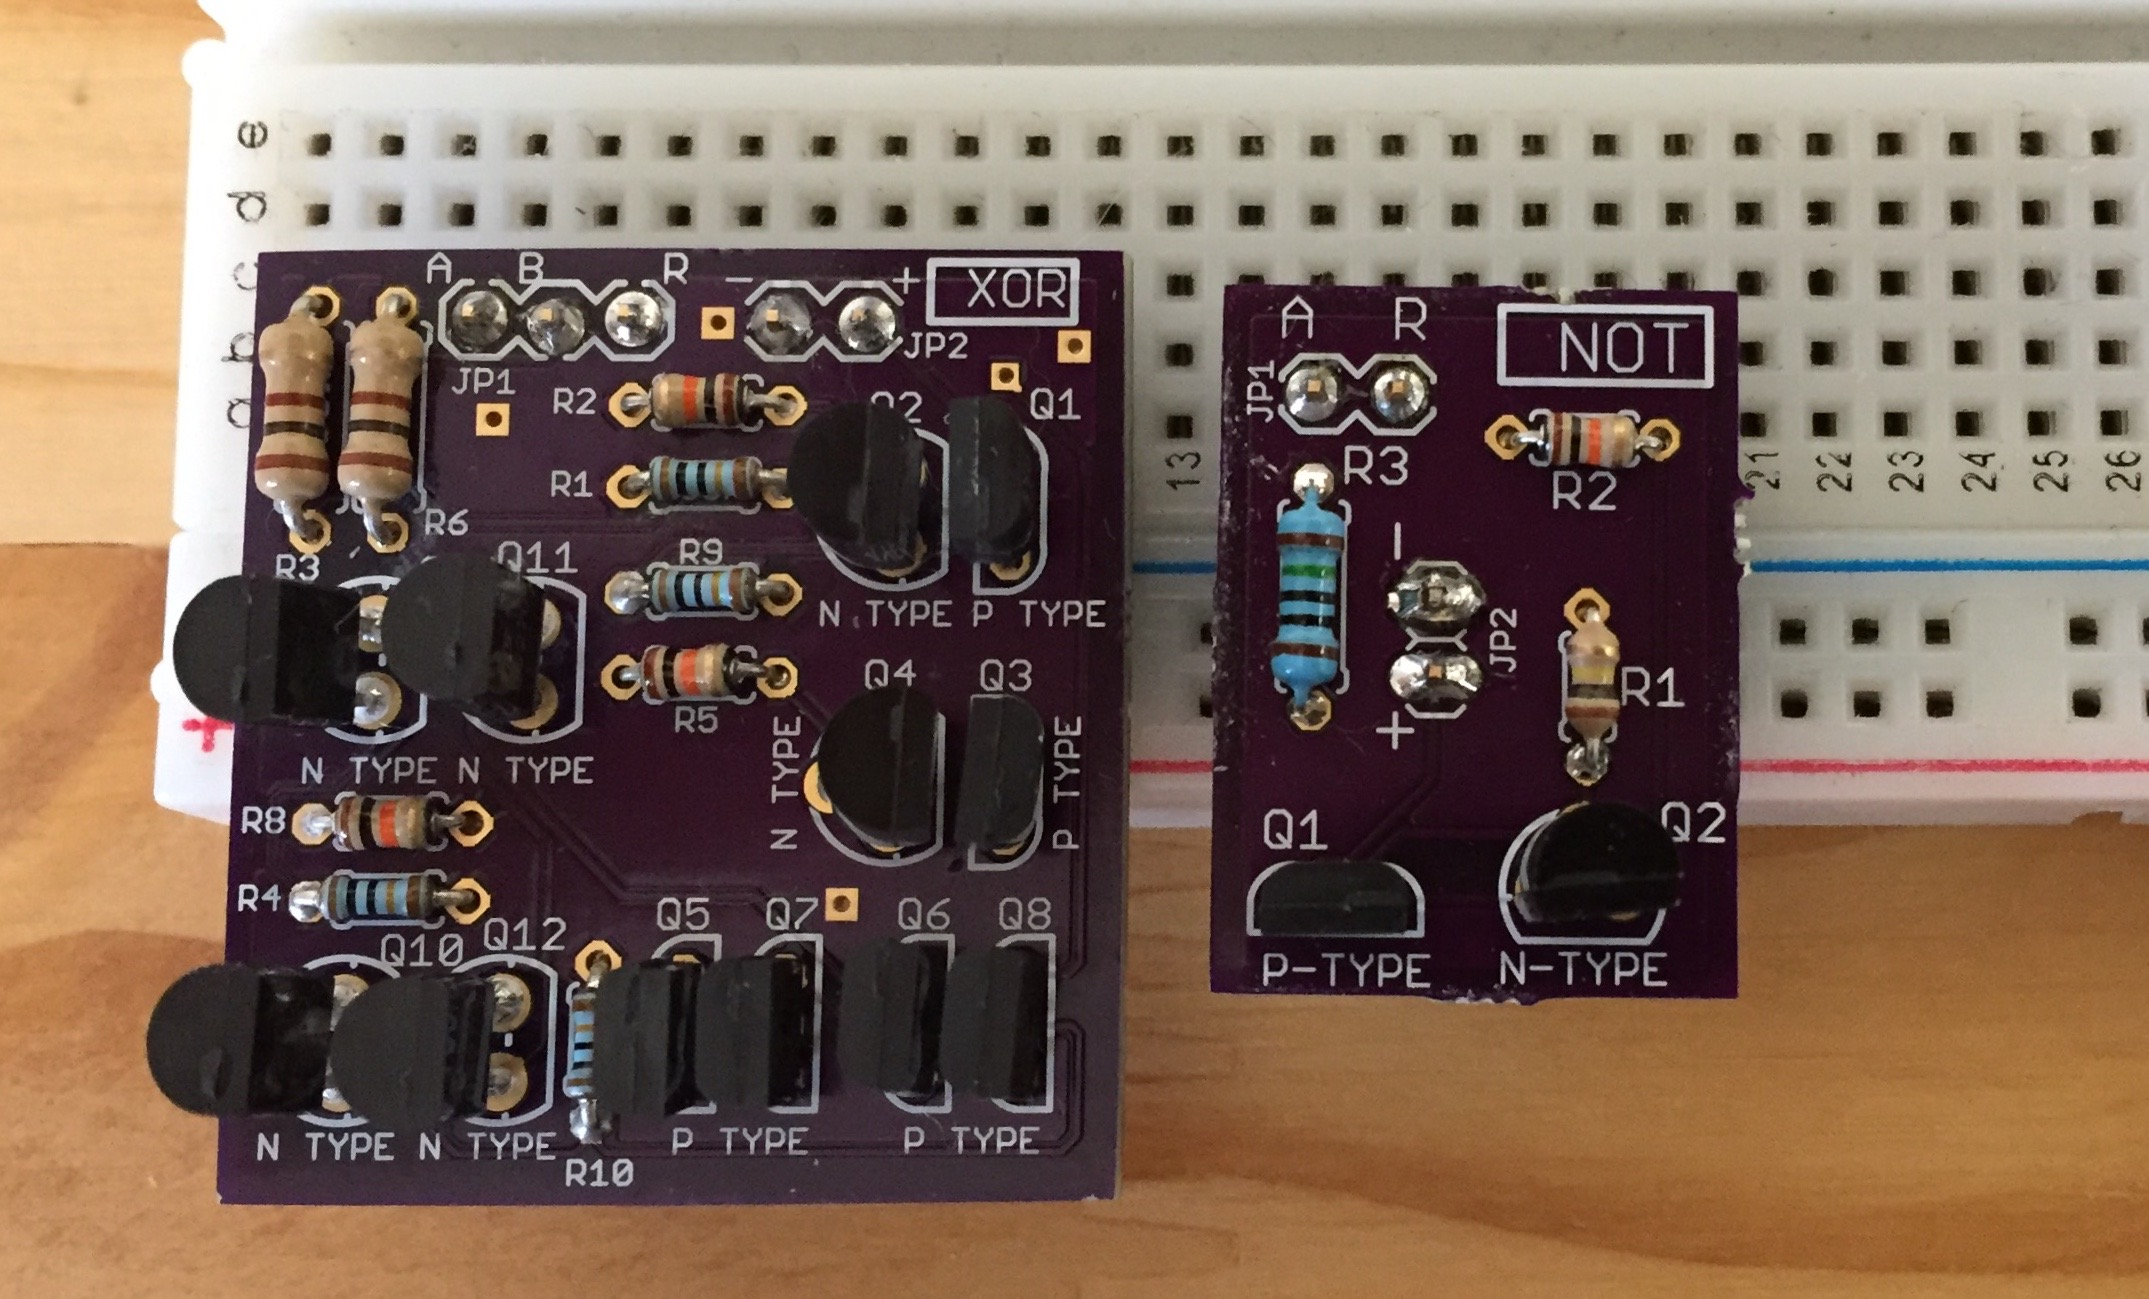
\includegraphics[scale=0.17]{XNORgate.jpg}
\caption{A discrete-transistor XOR and NOT gate. Tying the output of the XOR gate to the input of the NOT gate makes the result of the NOT gate an XNOR of the original two XOR gate inputs---answering the question ``are the two inputs equal?"}
\end{center}
\end{figure}

\clearpage


%---------------------------
\newpage
\section*{Memory}
%---------------------------

Logic circuits need to store the numbers they are working with in order to do more than one thing. Central Processing Units (CPUs), Arithmetic Logic Units (ALUs) or Floating-Point Units (FPUs) each work with numbers, and need to fetch them from somewhere and put them somewhere when they are done. The ``somewhere" is \emph{memory}. Keeping with the use of binary math and binary logic, a high voltage would be a 1 and a low voltage would be a 0. Through the use of these little stored charges, computers can keep track of many, many pieces of information. No matter what the circuits are doing, everything being stored is composed of some count of zeros and ones. 

There have been \emph{many} forms of memory through the years, including punched paper cards, and even a wiggly wire! The most common memory these days is a circuit made up of six transistors, or one transistor and a capacitor or two. Computers read eight, sixteen, 32, or 64 bits at a time from a row of memory and pass the number, or the instructions, from memory on to be processed.

One type of computer memory, called \emph{static RAM}, uses six transistors per bit instead of one transistor and a capacitor for bit (as used in dynamic ram, the main memory for the computer), so it's bulky, but it's also faster. To store one bit with 6 transistors is also expensive so SRAM is mostly used for very important memory, like the memory very close to the core of the computer processor. Have a look at Figure \ref{fig:sram}\footnote{Diagram and supporting information adapted from {\color{webblue}\href{https://en.wikipedia.org/wiki/Static_random-access_memory}{Wikipedia}} and {\color{webblue}\href{https://www.entner.net/sites/default/files/diss-entner-final-v1.pdf}{Robert Entner's dissertation}}.}, 
which is pretty complicated, but if you understand how the two types of transistors are turned on and off, it will make sense. To keep this diagram simple, no resistors are shown. If you look closely at the $Q_1$/$Q_2$ and $Q_3$/$Q_4$ transistors, you can see that they are acting like inverters (that is, each pair makes a NOT gate). When WL (the ``word line") goes high, $Q_5$ and $Q_6$ open up, allowing access to the single bit stored in $BL$ and the inverse of that bit in $\overline{BL}$. 

% TODO add a simpler diagram here, substituting NOT gate symbols for the twin CMOS NOT gates.

\begin{figure}[h!]
\begin{center}
\newcommand*\low[1]{\overline{#1}}

\begin{circuitikz}

\draw 
% Vdd:
%	(4,5) node[vdd](vdd){}
	(2,5) node[circ](vdd1) {}
	(6,5) node[circ](vdd2) {}	
    (4,5) node[above] {{\color{red}$V_{dd}$}} % Vdd
    (1.5,5) |- (6.5,5)

% GND
	(2,0) node[circ](gnd1) {}
	(6,0) node[circ](gnd2) {}
    (4,0) node[ground](ground){}
    (1.5,0) |- (6.5,0)

% Bit Line nodes:
	(0,2.25) node[circ](bllow) {}
	(0,1) node[left] {{\color{red}$\low{BL}$}} % BL low
	(8,2.75) node[circ](blhigh) {}
	(8,1) node[right] {{\color{red}$BL$}} % BL

% Bit Line:
	(0,0) |- (0,6)
	(8,0) |- (8,6)

% Word Line:
	(1,6) node[circ](wlgate1){} 
	(4,6) node[above] {{\color{red}$WL$}} % WL label
	(0.5,6) |- (7.5,6)
	(7,6) node[circ](wlgate2){}

% Two inverters:

% 2 P-type FETs:
	(2,4) node[pmos, emptycircle, xscale=-1](Q2){}
	(1.5,4) node[above]{$Q_2$}
	(6,4) node[pmos, emptycircle](Q4){$Q_4$}
	
% 2 N-type FETs:
	(2,1) node[nmos, xscale=-1](Q1){}
	(1.5,1) node[above]{$Q_1$}
	(6,1) node[nmos](Q3){$Q_3$}


% Word line gate N-type FETs:
	(1,2.25) node[nmos, rotate=-90](Q5){}
	(0.5,3.0) node[above]{$Q_5$}
	
	(7,2.75) node[nmos, rotate=-90](Q6){}
	(7.5,3.45) node[above]{$Q_6$}

% Bit Line FET nodes:
 (6, 2.75) node[circ] (m6Q1){}
 (2, 2.25) node[circ] (m5Q1){}
 
 (2.98,2.75) node[circ] (m6q2){}
 (5.01,2.25) node[circ] (m5q2){}

% Nets:
 (wlgate1) |- (Q5.G)
 (wlgate2) |- (Q6.G)

 (vdd1) |- (Q2.S)
 (vdd2) |- (Q4.S)

 (Q1.S) |- (gnd1)
 (Q3.S) |- (gnd2)

 (Q1.D) |- (Q2.D)
 (Q3.D) |- (Q4.D)
 
 (Q2.G) |- (Q1.G)
 (Q4.G) |- (Q3.G)
 
 (Q6.S) |- (2.97,2.75)
 (Q5.D) |- (5.01,2.25)

 (bllow) |- (Q5.S)
 (blhigh) |- (Q6.D)
;
\end{circuitikz}
\caption{A static ram cell.} 
\label{fig:sram}
\end{center}
\end{figure}

